Using the Madison, Wisconsin, Police Department data in Table 5.8, construct individual
$\bar{X}$ charts for $x_{3} = \text{holdover hours}$ and $x_{4} = \text{COA hours}$. Do these individual process
characteristics seem to be in control? (That is, are they stable?) Comment.

\begin{align*}
    \text{Upper control limit (UCL)} = \bar{\bar{x}} + \text{3(standard deviation)} \\
    \text{Lower control limit (LCL)} = \bar{\bar{x}} - \text{3(standard deviation)}
\end{align*}
We have individual observations, $\bar{\bar{x}} = \bar{x}$.

\begin{figure}[H]
    \centering
    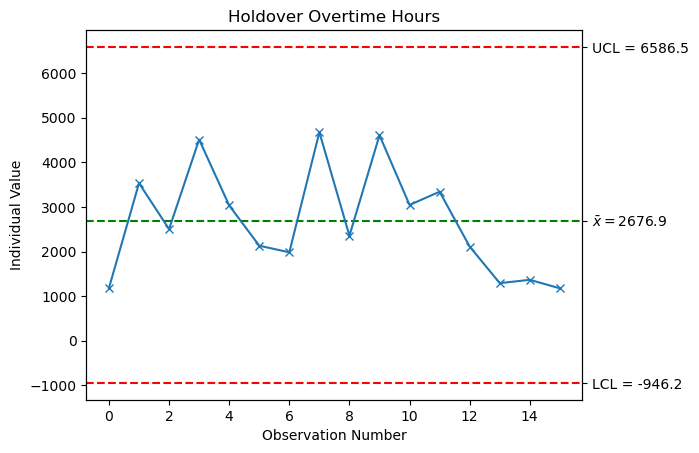
\includegraphics[scale=0.65]{./python/chapter-5/Question-5-24-Holdover.png}
\end{figure}

\begin{figure}[H]
    \centering
    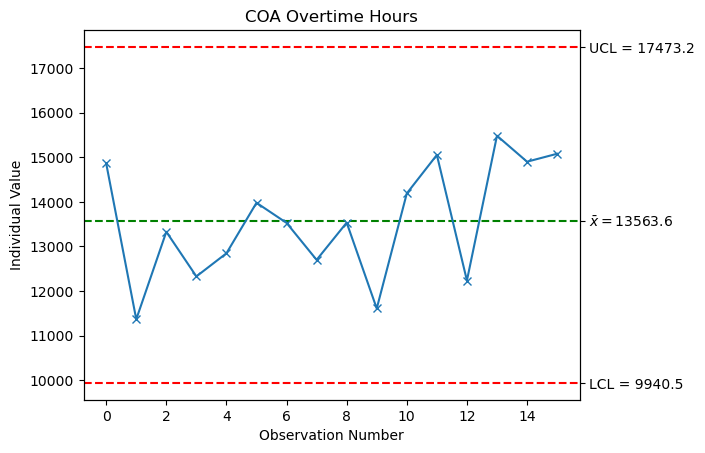
\includegraphics[scale=0.65]{./python/chapter-5/Question-5-24-COA.png}
\end{figure}

Both plots show all of the data within the 3 standard deviation bounds, so the process is stable and in control for both variables over the time the data was collected.